\documentclass[15pt,a5paper,reqno]{article}
\usepackage{hyperref}
\usepackage[warn]{mathtext}
\usepackage[utf8]{inputenc}
\usepackage[T2A]{fontenc}
\usepackage[russian]{babel}
\usepackage{amssymb, amsmath, multicol}
\usepackage{graphicx}
\usepackage[shortcuts,cyremdash]{extdash}
\usepackage{wrapfig}
\usepackage{floatflt}
\usepackage{lipsum}
\usepackage{verbatim}
\usepackage{concmath}
\usepackage{euler}
\usepackage{xcolor}
\usepackage{etoolbox}
\usepackage{fancyhdr}
\usepackage{subfiles}
\usepackage{enumitem}
\usepackage{amsthm}
\usepackage{indentfirst}
\usepackage{import}

\DeclareMathOperator{\sign}{sign}

\RequirePackage[ left     = 1.5cm,
  right    = 1.5cm,
  top      = 2.0cm,
  bottom   = 1.25cm,
  includefoot,
  footskip = 1.25cm ]{geometry}
\setlength    {\parskip}        { .5em plus .15em minus .08em }
%\setlength    {\parindent}      { .0em }
\renewcommand {\baselinestretch}{ 1.07 }

\fancyhf{}

\renewcommand{\footrulewidth}{ .0em }
\fancyfoot[C]{\texttt{\textemdash~\thepage~\textemdash}}
\fancyhead[R]{\hfilШурыгин}

\makeatletter
\patchcmd\l@section{%
  \nobreak\hfil\nobreak
}{%
  \nobreak
  \leaders\hbox{%
    $\m@th \mkern \@dotsep mu\hbox{.}\mkern \@dotsep mu$%
  }%
  \hfill
  \nobreak
}{}{\errmessage{\noexpand\l@section could not be patched}}
\makeatother
\parindent = 1cm % отступ при красной строке⏎
\pagestyle{fancy}    
\renewcommand\qedsymbol{$\blacksquare$}

\newcommand{\when}[2]{
  \left. #1 \right|_{#2} \hspace
}
\renewcommand{\kappa}{\varkappa}
\RequirePackage{caption2}
\renewcommand\captionlabeldelim{}
\newcommand*{\hm}[1]{#1\nobreak\discretionary{}

\DeclareSymbolFont{T2Aletters}{T2A}{cmr}{m}{it}
{\hbox{$\mathsurround=0pt #1$}}{}}
% Цвета для гиперссылок
\definecolor{linkcolor}{HTML}{000000} % цвет ссылок
\definecolor{urlcolor}{HTML}{799B03} % цвет гиперссылок
 
\hypersetup{pdfstartview=FitH,  linkcolor=linkcolor,urlcolor=urlcolor, colorlinks=true}


%\setcounter{secnum[utf8x]depth}{0}

\begin{document}

% НАЧАЛО ТИТУЛЬНОГО ЛИСТА
\begin{center}
  {\small ФЕДЕРАЛЬНОЕ ГОСУДАРСТВЕННОЕ АВТОНОМНОЕ ОБРАЗОВАТЕЛЬНОЕ\\ УЧРЕЖДЕНИЕ ВЫСШЕГО ОБРАЗОВАНИЯ\\ МОСКОВСКИЙ ФИЗИКО-ТЕХНИЧЕСКИЙ ИНСТИТУТ\\ (НАЦИОНАЛЬНЫЙ ИССЛЕДОВАТЕЛЬСКИЙ УНИВЕРСИТЕТ)\\ ФИЗТЕХ-ШКОЛА РАДИОТЕХНИКИ И КИБЕРНЕТИКИ}\\
  \hfill \break
  \hfill \break
  \hfill \break
  \Huge{Тепловое излучение}\\
\end{center}

\hfill \break
\hfill \break
\hfill \break
\hfill \break
\hfill \break
\hfill \break

\begin{flushright}
  \normalsize{Работу выполнил:}\\
  \normalsize{\textbf{Шурыгин Антон Алексеевич, группа Б01-909}}\\
\end{flushright}

\begin{center}
  \normalsize{\textbf{Долгопрудный, 2021}}
\end{center}


\thispagestyle{empty} % выключаем отображение номера для этой страницы

% КОНЕЦ ТИТУЛЬНОГО ЛИСТА

\newpage
\thispagestyle{plain}
\tableofcontents
\thispagestyle{plain}
\newpage

\paragraph{Цель работы:} проведение измерения температуры оптическим пирометром с исчезающей нитью и термопарой, определение постоянных Планка и Стефана-Больцмана, исследование излучение накалённых тел с различной испускательной способностью.
\paragraph{Оборудование:} оптический пирометр, модель абсолютно чёрного тела, образцы колец, вольфрамовая лампа, неоновая лампа, блок питания, цифровые вольтметры.


\section{Теория}

Для измерения температуры разогретых тел, удалённых от наблюдателя, применяют методы оптической пирометрии, основанные на использовании зависимости испускательной способности исследуемого тела от температуры. Различают три температуры, функционально связанные с истинной термодинамической температурой и излучательной способностью тела: радиационную $T_{rad}$, цветовую $T_{col}$ и яркостную $T_{b_r}$.
В работе измеряется яркостная температура.

\textbf{Яркостная температура} - это температура абсолютно чёрного тела, при которой его спектральная испускательная способность равна спектральной испускательной способности исследуемого тела при той же длине волны.
 Измерение яркостной температуры раскалённого тела производится при помощи оптического пирометра с исчезающей нитью, основанного на визуальном сравнении яркости раскалённой нити с яркостью изображения исследуемого тела. \par
Яркостная температура тела всегда ниже его термодинамической температуры. Это связано с тем, что любое нечёрное тело излучает меньше, чем АЧТ при той же температуре. Зависимость между яркостной и термодинамической температурами вольфрама приведена на рис. 1

\begin{figure}[h]
    \centering
    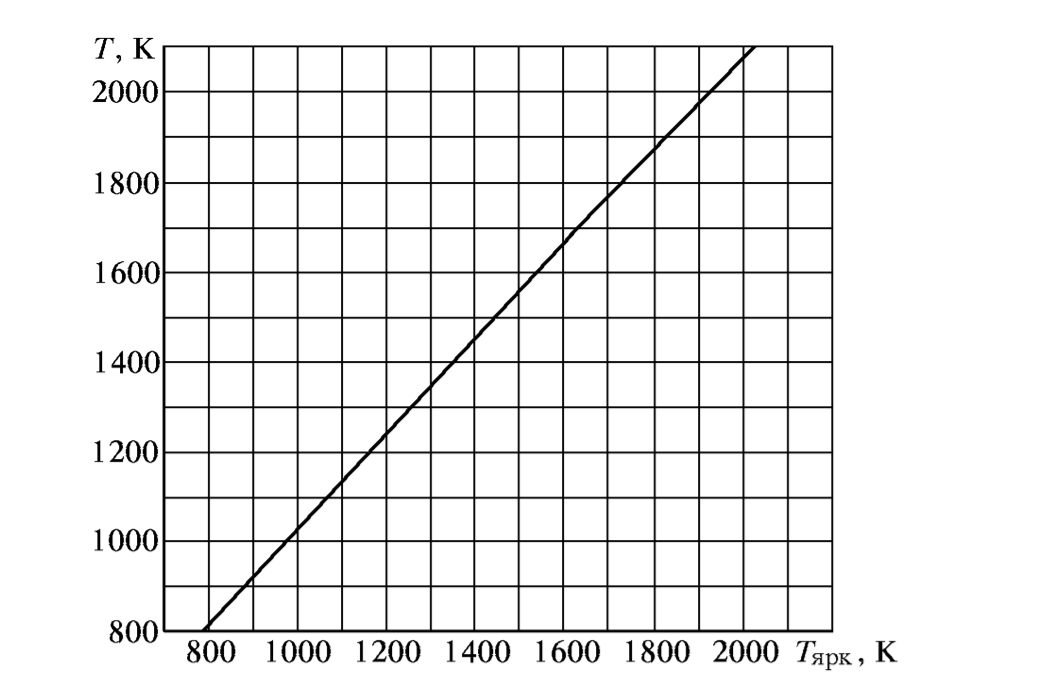
\includegraphics[width=10cm]{pics/lab_5_8_1_theor.png}
    \caption{График зависимости $T = f(T_{br}$ для вольфрам}
    \label{fig:vac}
\end{figure}

По результатам измерений мощности излучения вольфрамовой нити можно судить о справедливости закона Стефана-Больцмана. Если бы нить излучала как АЧТ, то баланс потребляемой и излучаемой энергии определялся бы соотношением 
\begin{equation}
    W = \sigma S (T^4 - T_0^4),
\end{equation}


где $W$ - потребляемая нитью электрическая мощность, $S$ - площадь излучающей поверхности нити, $T$ - температура нити, $T_0$ - температура окружающей среды. Однако вольфрамовая нить излучает как серое тел, и излучение её ослаблено по сравнению с АЧТ в $\varepsilon_T$ раз для любой волны при данной температуре тела Т. Тогда предположив, что нить излучает как серое тело и с учётом того, что $T_0 \ll T$, выражение (1) можно переписать в виде

\begin{equation}
    \label{SteffBolcmn}
    W = \varepsilon_T S \sigma T^4
\end{equation}

В справедливости закона Стефана-Больцмана можно убедиться, построив график зависимости $W(T)$ в логарифмическом масштабе и по углу наклона определить показатель степени $n$ исследуемой температурной зависимости. В пределах погрешности показатель степени должен быть близок к четырём. \par
Также из формулы (2) можно определить постоянную Стефана-Больцмана.

\section{Экспериментальная установка}

\begin{figure}[h]
    \centering
    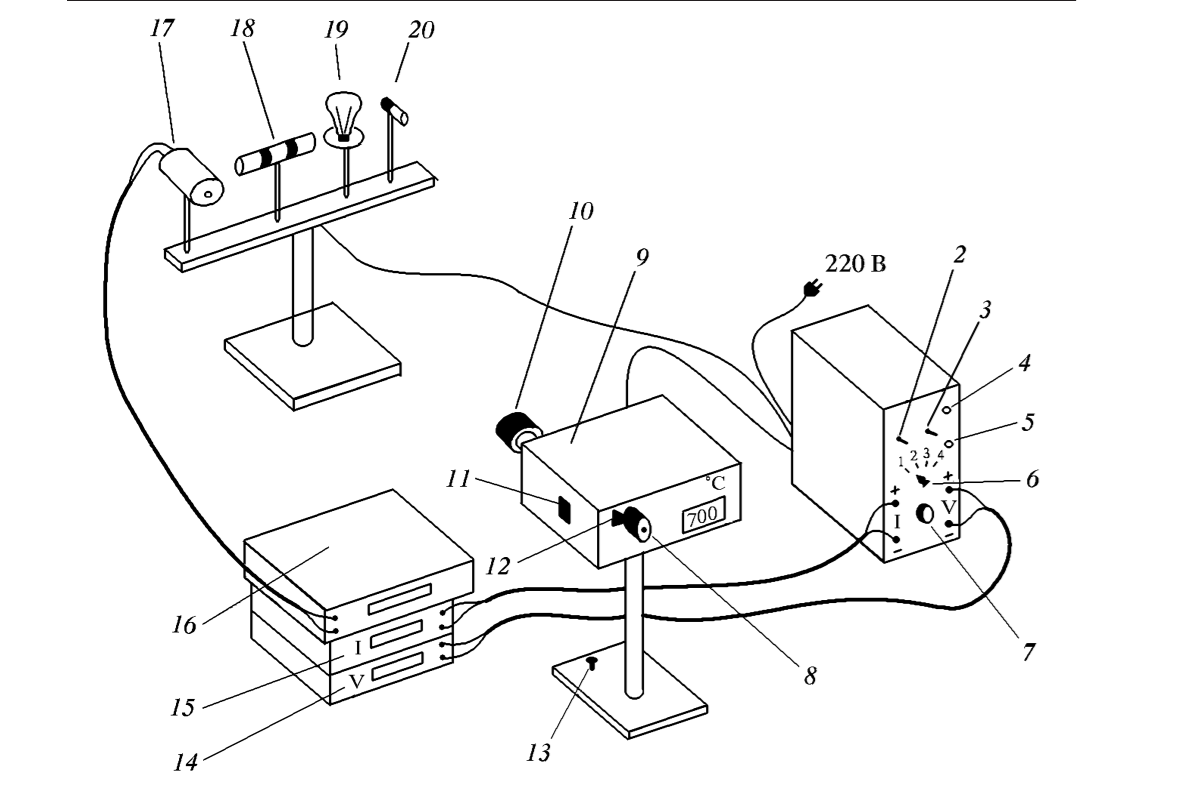
\includegraphics[width=11cm]{pics/lab_5_8_1_scheme.png}
    \caption{Схема экспериментальной установки: 1 - блок питания; 2 - тумблер включения питания образцов; 3 - тумблер нагрева нити пирометра; 4 - кнопка "Нагрев нити"; 5 - кнопка "охлаждение нити"; 6 - тумблер переключения образцов; 7 - регулятор мощности нагрева образцов; 8 - окуляр пирометра; 9 - корпус пирометра; 10 - объектив пирометра; 11 - переключение диапазонов; 12 - ручка смещения красного светофильтра; 13 - регулировочный винт; 14 - вольтметр (напряжение на лампе накаливания); 15 - амперметр (ток через образцы); 16 - вольтметр в цепи термопары; 17 - модель АЧТ; 18 трубка с кольцами из материалов с различной излучательной способностью; 19 - лампа накаливания; 20 - неоновая лампочка}
    \label{scheme}
\end{figure}

Исследуемые в работе образцы:
\begin{itemize}
    \item \textbf{модель абсолютно чёрного тела} - керамическая трубка, закрытая с одного конца и окружённая для теплоизоляции внешним кожухом. Температура в трубке измеряется с помощью термопары хромель-алюмель
    \item \textbf{керамическая трубка с набором колец из различных материалов}, нагреваемая изнутри нихромовой спиралью. Материалы колец имеют различную излучательную способность
    \item \textbf{вольфрамовая нить электрической лампочки}
\end{itemize}


\section{Ход работы и обработка данных}

\subsection{Изучение работы оптического пирометра}

С помощью пирометра измеряется температура модели АЧТ и проводится сравнение её значения  со значением температуры, измеренной при помощи термопарного термометра.
\begin{enumerate}
    \item Настроим пирометр, прогреем его нить. Прогреем модель АЧТ.
    \item Введём красный светофильтр пирометра. Изменяя ток через нить пирометра, добьёмся исчезновения нити на фоне изображения раскалённой поверхности дна АЧТ. Проверим корректность измерений: температура на пирометре не должна сильно отличаться от температуры АЧТ, измеренной термопарой. Результаты измерений занесём в таблицу 1.

    \begin{table}[h!]
        \centering
        \begin{tabular}{| c | c | c | c | c |}
\hline
$U, mV$ & $T_{room}, K$ & $T, K$ & $T_{br}, K$ & $ \sigma_{T}, K$\\
\hline
$39920$ & $298$ & $973,66$ & $1000$ & $ 28 $\\
\hline
\end{tabular}

        \caption{: настройка пирометра}
    \label{tb_1}
    \end{table}

Видим, что разница в показаниях приборов не превышает 3\%
\end{enumerate}

\subsection{Измерение яркостной температуры тел}
Показывается, что разные тела, накалённые до одинаковой термодинамической температуры, имеют различную яркостную температуру


\subsection{Проверка закона Стефана-Больцмана}
\begin{enumerate}

\item Постепенно увеличивая накал нити лампы, начиная со слабого тёмно-красного накала до 1900$^{\circ}$C, будем измерять пирометром яркостную температуру нити, а также значение силы тока и напряжения на ней. Результаты измерений занесём в таблицу 2. Определим также по значениям яркостной температуры нити её термодинамическую температуру, используя рис. 1.
    
\begin{table}[h!]
        \centering
        \begin{tabular}{| c | c | c | c | c |}
\hline
$\theta,^{\circ}$ & $U(I)$ & $V_{ФЭ}$ & $\sigma_{U(I)}$ & $\sigma_{V_{ФЭ}}$\\
\hline
$2404$ & $0,036$ & $0,302$ & $0,0004$ & $0,003$\\
\hline
$$ & $0,032$ & $0,262$ & $0,0004$ & $0,003$\\
\hline
$$ & $0,027$ & $0,202$ & $0,0004$ & $0,003$\\
\hline
$$ & $0,02$ & $0,121$ & $0,0004$ & $0,003$\\
\hline
$$ & $0,016$ & $0,039$ & $0,0004$ & $0,003$\\
\hline
$$ & $0,009$ & $-0,062$ & $0,0004$ & $0,003$\\
\hline
$$ & $0,006$ & $-0,162$ & $0,0004$ & $0,003$\\
\hline
$$ & $0$ & $-0,303$ & $0,0004$ & $0,003$\\
\hline
\end{tabular}

        \caption{: данные для графика}
    \label{tb_2}
\end{table}

\item Представим зависимость $W=f(T)$ в логарифмическом масштабе как $\ln(W) = \ln(\varepsilon_T \sigma S) + n \ln(T)$ По углу наклона графика можно определить показатель степени температуры в законе Стефана-Больцмана. 

\[ y = 3,83x - 23,71 \] 

\begin{table}[h!]
    \centering
    \begin{tabular}{| c | c |}
\hline
$ln(T_{term})$ & $ln(P)$\\
\hline
$6,82$ & $2,43$\\
\hline
$6,96$ & $2,88$\\
\hline
$7,05$ & $3,42$\\
\hline
$7,15$ & $3,73$\\
\hline
$7,22$ & $3,98$\\
\hline
$7,31$ & $4,25$\\
\hline
$7,38$ & $4,48$\\
\hline
$7,4$ & $4,72$\\
\hline
$7,48$ & $4,88$\\
\hline
$7,51$ & $5,1$\\
\hline
$7,55$ & $5,29$\\
\hline
\end{tabular}

    \caption{: данные для графика}
\label{tb_3}
\end{table}

\textbf{Оценка прогрешностей}:

\begin{itemize}
    \item \textbf{Логарифма температуры:}
      
    \[  \sigma_{ln(T)} = \frac{\sigma_T}{T} \]

    \item \textbf{Мощности:}
    
    \[ \sigma_{P} = \sigma_{UI} = \sigma_P \cdot \sqrt{\left( \frac{\sigma_I}{I} \right)^{2}  +  \left( \frac{\sigma_U}{U} \right)^{2}} \]
    
    \item \textbf{Логарифма от мощности:}
    
    \[ \sigma_{ln(P)} = \frac{\sigma_P}{P}\]

    \item \textbf{Постоянной Стефана-Больцмана:}
    
    \[ \sigma_{\sigma} = \sigma \sqrt{\left( \frac{\sigma_P}{P} \right)^{2}  +  16\cdot\left( \frac{\sigma_T}{T} \right)^{2}   }   \]
    
    \item \textbf{Постоянной Планка:}

    \[ \sigma_h = h \frac{3\sigma_{\sigma}}{2\sigma} \]
\end{itemize}


\begin{figure}[h]
    \centering
    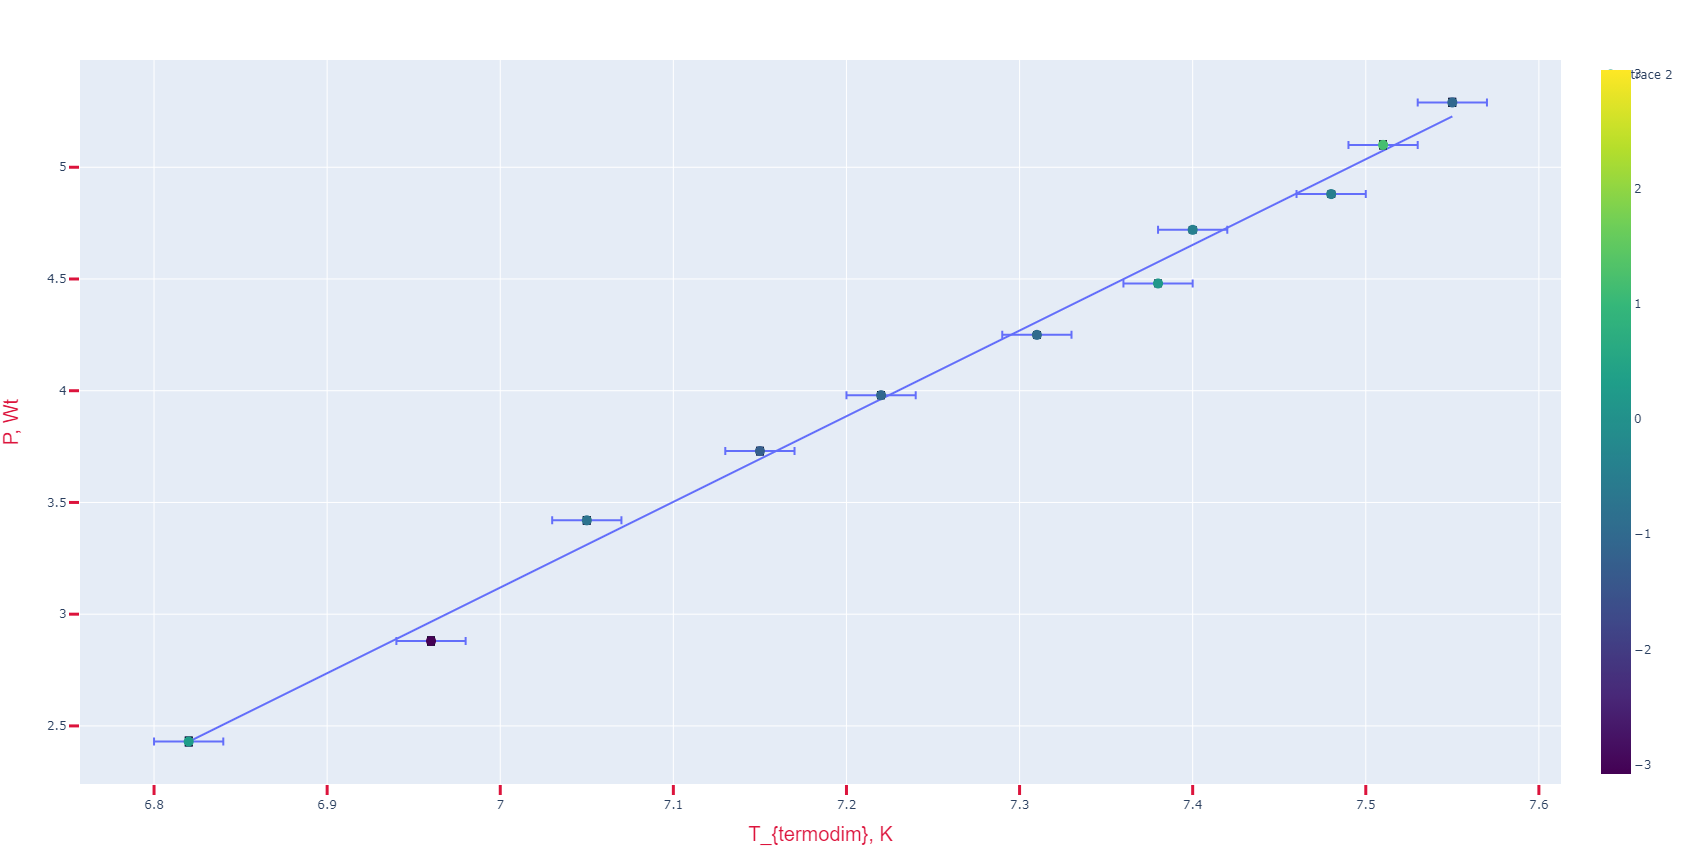
\includegraphics[width=\textwidth]{pics/graph_5_8_1.png}
    \caption{Зависимость мощности лампы от её термодинамической температуры, логарифмический масштаб}
    \label{graph}
\end{figure}

\item Определим постоянную Стефана-Больцмана для трех значений термодинамической температуры $T_{term}$ по формуле:

\[  \sigma = \frac{W}{\varepsilon_T S T^4} =   \]

\begin{itemize}
    \item $T_1 = 1770$ K $\Rightarrow \sigma_1 = \frac{W}{\varepsilon_T S T_{1}^{4}} \approx (8,3 \pm 0,2) \cdot 10^{-7} \frac{Вт}{м \cdot K^{-4}}  $
    \item $T_2 = 1820$ K $\Rightarrow \sigma_2 = \frac{W}{\varepsilon_T S T_{2}^{4}} \approx (9,4 \pm 0,3)  \cdot 10^{-7} \frac{Вт}{м \cdot K^{-4}}  $
    \item $T_3 = 1900$ K $\Rightarrow \sigma_3 = \frac{W}{\varepsilon_T S T_{3}^{4}} \approx (10,9 \pm 0,3) \cdot 10^{-7} \frac{Вт}{м \cdot K^{-4}}  $
\end{itemize}


Также можно определить постоянную Стефана-Больцмана, используя построенный график зависимости $\ln(W) = \ln(\varepsilon_T \sigma S) + n \ln(T)$
По графику видно, что $n \approx 3,81 \approx 4$, что лучше соответствует теории, нежели результаты выше.



\[  \sigma_{th} = 5.67 \cdot 10^{-8}  \frac{\text{Вт}}{\text{м}^2 \cdot \text{K}^{4}} \]
\item Оценим значение постоянной Планка, взяв значения из приближения двойного логарифмического масштаба, т.к. он показал более точный результат оценки константы Стеффана-Больцмана.


При $T_{term} \approx 1900 K$, $P \approx 186,3$ Вт $\Rightarrow$ $\sigma \approx 91 \cdot 10^{-8} \frac{\text{Вт}}{\text{м}^2 \cdot \text{K}^{4}}   $ 

\[ h = \sqrt[3]{\frac{2 \pi^5 k_B^4}{15 c^2 \sigma}} \approx  (5,6 \pm 0,3) \cdot 10^{-35}  \text{ Дж $\cdot$с} \]

\end{enumerate}

\subsection{Измерение яркостной температуры неоновой лампочки}
Термодинамическая температура неоновой лампочки примерно равна комнатной, и не соответствует её яркостной температуре ($\approx$ 830$^{\circ}$C). Дело в том, что неоновая лампочка в принципе не является моделью абсолютно чёрного или серого тела, и её излучение носит совершенно другую природу (переход электронов между энергетическими уровнями). То, что её свет имеет такой же цвет, что и нагретое АЧТ - совпадение.

\section{Вывод}
В ходе работы было изучено тепловое излучение модели абсолютно чёрного тела и моделей серых тел - колец из различных материалов и вольфрамовой нити. Было проведено ознакомление с принципом работы оптического пирометра - в ходе его настройки и работы с моделью АЧТ выяснилось, что разность показаний пирометра и действительной температурой составляет до 10\% . 
Этот фактор мог быть причиной того, что в ходе работы не было подтверждено выполнение закона Стефана-Больцмана. \par
При проведении работы мы наблюдали, что для различных материалов с одинаковой термодинамической температурой их яркостная температура может не совпадать. Это связано с различием коэффициента спектрального поглощения этих материалов. \par
В работе было предложено проверить справедливость закона Стефана-Больцмана ($W \propto T^4$). К сожалению, такую зависимость получить не удалось - значение степени при Т, определённое в работе, составляло 2.68 $\approx$ 3. Возможные причины этого несовпадения:
\begin{itemize}
    \item сильный теплоотвод от нити
    \item ошибка в показаниях пирометра
    \item ошибка в визуальном определении яркости
\end{itemize}
Также по результатам измерений была оценена постоянная Стефана-Больцмана двумя способами - непосредственно используя формулу (2) и используя график зависимости $W(t)$ в логарифмическом масштабе. Второй способ оказался более точным:

%\begin{center}
%    $\sigma_1 = 0.158\cdot 10^{-12}$ Вт/(см$^2 \cdot$ K$^4$) \\
%    $\sigma_2 = 3.335 \cdot 10^{-12}$ Вт/(см$^2 \cdot$ K$^4$) \\
%     $\sigma_t_h = 5.67\cdot 10^{-12}$ Вт/(см$^2 \cdot$ K$^4$)
%\end{center}

Наконец, в ходе работы с помощью пирометра была определена "яркостная температура" неоновой лампочки, не являющейся моделью АЧТ. Эта яркостная температура не совпадает с термодинамической
\end{document}